\section{Competition Outlines}

\subsection{Flight Arena}
\begin{enumerate}
	\item{The flight arena will have a size of 6m height, 20m length, and 18m width}
	\item{The flight arena will be indoors. Expect bad GPS signal and don't soley rely on gps for you state estimation. Details on positioning using fudicial marker are described in the technical section.}
	\item{The map coordinate frame is a right handed coordnate frame, which is attached to the middle line with the z axis pointing upwards the x axis is pointing to the middle of the field.}
\end{enumerate}
\begin{figure}[H]
	\centering
	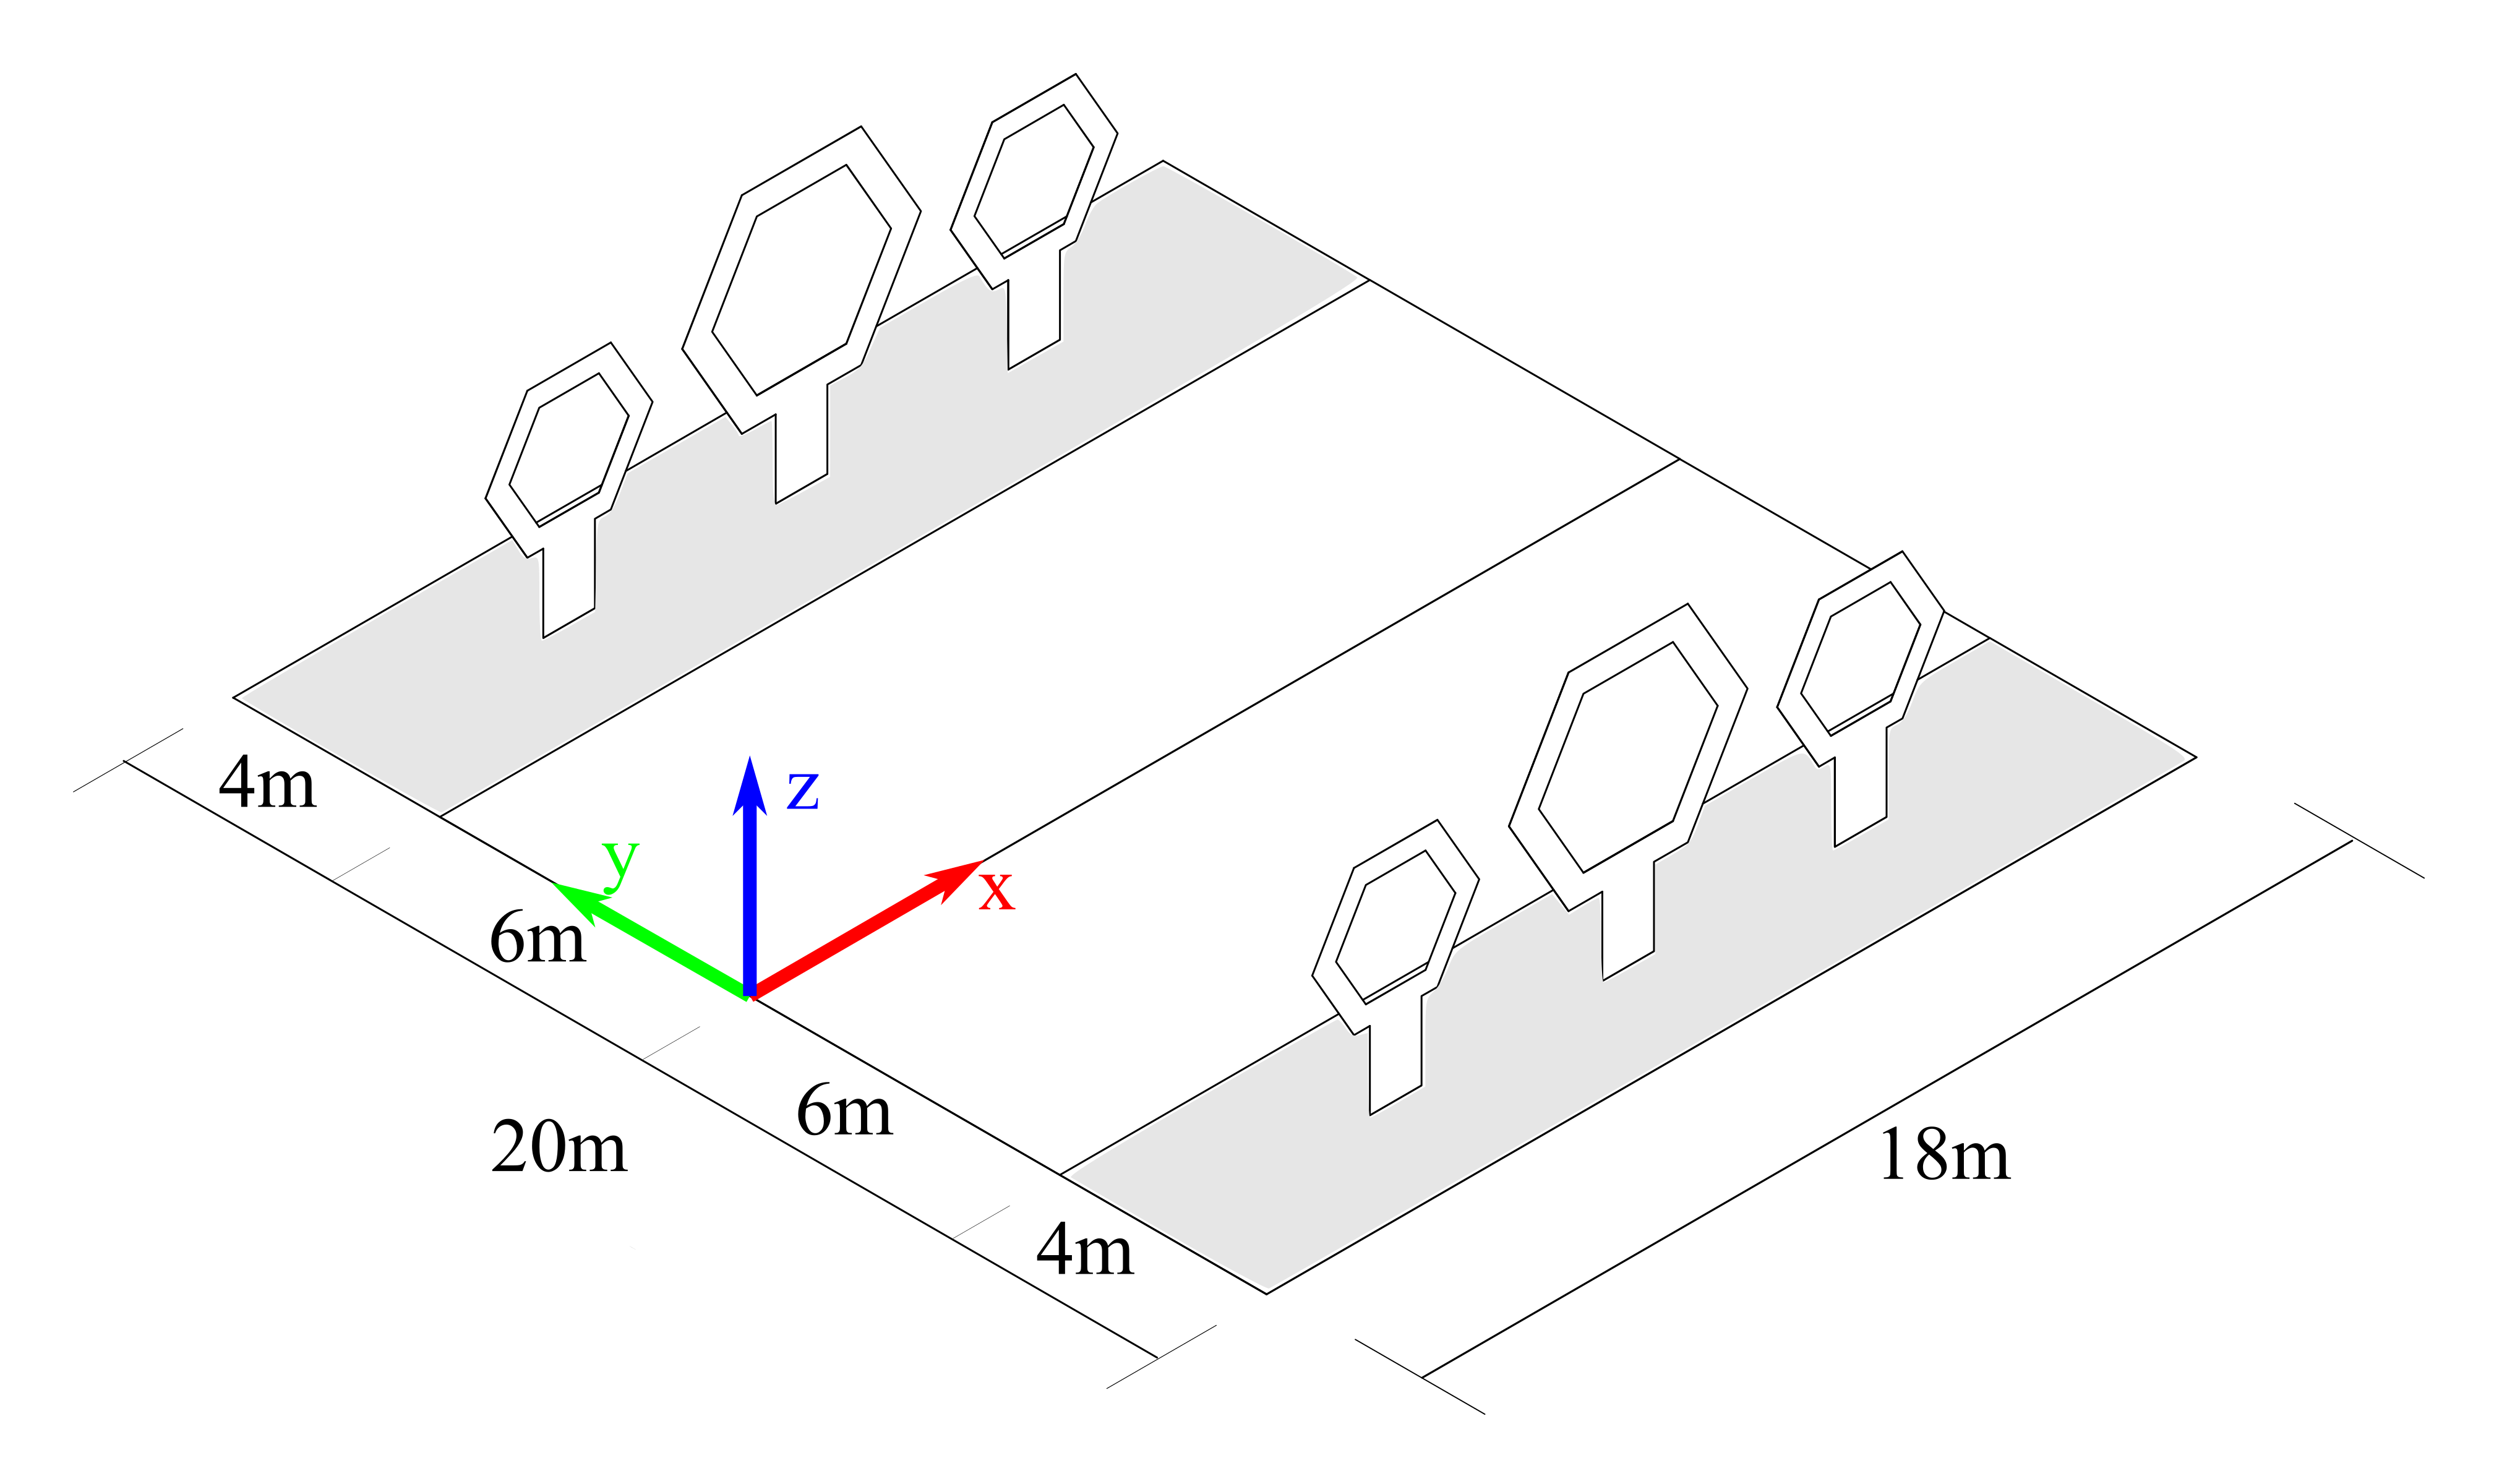
\includegraphics[width=400pt]{SDC_FlightArena.png}
	\caption{Flight Arena Dimensions}
	\label{fig:flight_arena}
\end{figure}
\subsection{Game Dynamics}
\begin{enumerate}
	\item{All drones of one team have to start in their own territory.}
	\item{\textcolor{red}{Drones need to activate hexagons by flying through them.}}
	\item{\textcolor{red}{There are 6 hexagons in total. 3 per team.}}
	\item{\textcolor{red}{The hexagon in the own territory are preactivated in the beginning of each halftime}}
	\item{\textcolor{red}{The game lasts 10 minutes}}
	\item{\textcolor{red}{The game is paused after 5 minutes and the sides are swapped.}}
	\item{\textcolor{red}{The goal is to activate as many hexagons as possible.}}
\end{enumerate}

\subsection{Rewards / Scoring}
\begin{enumerate}
	\item{\textcolor{red}{A team can earn max 80 points. 60 points can be scored during the game and 20 points are awarded by the jury.}}
	\item{\textcolor{red}{You can earn 1 point per minute for each hexagon that is activated. (Each second will be counted as 1/60 point)}}
	\item{\textcolor{red}{The jury will award up to 20 points for the presentation and the technical implementation.}}
	\item{\textcolor{red}{The team with the most points wins.}}
\end{enumerate}

\subsection{Teams}
\begin{enumerate}
	\item{Up to 5 team members per team}
	\item{New team members are allowed to join but need to be registered with brigk.}
\end{enumerate}

\subsection{Reimbursement}
\begin{enumerate}
	\item{\textcolor{red}{Up to 1000€ for drone parts}}
	\item{\textcolor{red}{Max 5 orders}}
\end{enumerate}

\subsection{Penalty and disqualification}
\begin{enumerate}
	\item{\textcolor{red}{Leaving the flight arena will be penalized with a deduction of 5 points.}}
	\item{\textcolor{red}{Starting the motors of the drones before the official start will be penalized with a deduction of 5 points }}
\end{enumerate}

\subsection{Intellectual property}
\begin{enumerate}
	\item{The IP stayes at the teams}
	\item{The teams are encouraged to open source their solutions. This can have an effect on the jury voting}
	\item{The teams are required to prepare a presentation and explain their solution with technical details on the implementation.}
\end{enumerate}

\subsection{Responsibilities}
\begin{enumerate}
	\item{\textcolor{red}{Each team must have a spotter}}
	\item{\textcolor{red}{Teams are responsible to virtually validate their solution}}
\end{enumerate}
